%adding TAIGA|Tunka data

% 11. Присоединение данных TAIGA (Tunka-133, HiSCORE) (как идея)
%         отличие тунки от каскада, черенки/сцинтиляторы
%         картинки с хмах
%         мэппинг данных
%
%         разделение гамма/кр тунка133 +

\begin{frame}{Tunka-133 and TAIGA HiScore}
%  \begin{columns}
%   \begin{column}
%   \begin{center}
%    \includegraphics[width=0.8\textwidth]{pics/tunka133_layot.pdf}
%   \end{center}
% 
%   \end{column}
%   \begin{column}
%    2
%   \end{column}
%  \end{columns}
\begin{itemize}
 \item TAIGA setups are located at the latitude as KASCADE;
 \item The possibility to scale  Tunka-133 and KASCADE-Grande was shown at:

W.D. Apel, et al. - Tunka-Rex and LOPES Collaborations, Phys. Lett. B 763 (2016) 179
\end{itemize}
% A comparison of the cosmic-ray energy scales of Tunka-133 and
% KASCADE-Grande via their radio extensions Tunka-Rex and LOPES
\end{frame}


\begin{frame}{KASCADE-TAIGA joint analysis}
\small
\begin{center}
    \begin{minipage}{0.55\textwidth}
     	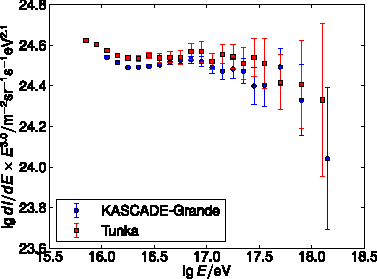
\includegraphics[width=1\textwidth]{pics/KG_tunka133_scales.pdf}
    \end{minipage}
%     \begin{minipage}{0.07\textwidth}
     $\longleftarrow$ 
%     \end{minipage}
\begin{minipage}{0.38\textwidth}	
  Energy spectra of cosmic rays from KASCADE-Grande and Tunka-133: normalized flux per energy.
      \end{minipage}
   
\end{center}

\begin{itemize}
 \item  With a systematic increase of
KASCADE-Grande energies by 4\% (or a corresponding decrease of Tunka-133 energies) 
the average flux per energy of both experiments can be brought to agreement
in this energy range.
\end{itemize}
% \end{minipage}
\end{frame}

\begin{frame}{Tunka-133 $\gamma$ - proton separation}
    \begin{center}
	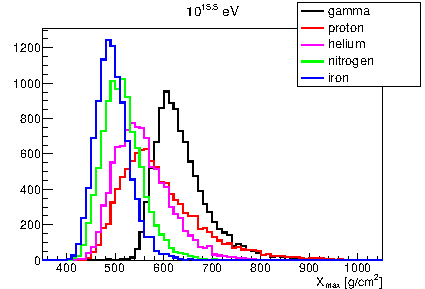
\includegraphics[width=0.8\textwidth]{pics/tunka_gamma_cr_diff.pdf}
	
      Distribution of $X_{max}$ for various primaries at $E = 10^{5.5} eV$.
    \end{center}
\end{frame}

